\documentclass[12pt,onecolumn]{article}
\usepackage[utf8]{inputenc} % UTF8 input encoding
\usepackage[T2A]{fontenc}   % T2A font encoding for Cyrillic script
\usepackage[russian]{babel} % Russian language support
\usepackage{listings}
\usepackage{float}
\usepackage{mathtools}
\usepackage{longtable}
\everymath{\displaystyle}
\usepackage{listings} 
\usepackage[usenames]{color}
\usepackage{geometry}
\geometry{
  a4paper,
  top=25mm, 
  right=15mm, 
  bottom=25mm, 
  left=15mm
}

\begin{document}
\setcounter{tocdepth}{4}
\begin{center}
    Федеральное государственное автономное образовательное учреждение высшего образования "Национальный Исследовательский Университет ИТМО"\\ 
    Мегафакультет Компьютерных Технологий и Управления\\
    Факультет Программной Инженерии и Компьютерной Техники \\
    
\includegraphics[scale=0.3]{image/itmo.jpg} % нужно закинуть картинку логтипа в папку с отчетом
\end{center}
\vspace{1cm}


\begin{center}
    \textbf{Лабораторная работа №1}\\
    по дисциплине\\
    \textbf{'Информационные системы и базы данных'}\\
    \textbf{Вариант 3893}
\end{center}

\vspace{2cm}

\begin{flushright}
  Выполнил Студент  группы P33102\\
  \textbf{Лапин Алексей Александрович}\\
  Преподаватель: \\
  \textbf{Блохина Елена Николаевна}\\
\end{flushright}

\vspace{6cm}
\begin{center}
    г. Санкт-Петербург\\
    2023г.
\end{center}

\newpage
\tableofcontents
\newpage

\section{Текст задания.}
Для выполнения лабораторной работы №1 необходимо:
\begin{enumerate}
  \item На основе предложенной предметной области (текста) составить ее описание. Из полученного описания выделить сущности, их атрибуты и связи.
  \item Составить инфологическую модель.
  \item Составить даталогическую модель. При описании типов данных для атрибутов должны использоваться типы из СУБД PostgreSQL.
  \item Реализовать даталогическую модель в PostgreSQL. При описании и реализации даталогической модели должны учитываться ограничения целостности, которые характерны для полученной предметной области.
  \item Заполнить созданные таблицы тестовыми данными.
\end{enumerate}
Для создания объектов базы данных у каждого студента есть своя схема. Название схемы соответствует имени пользователя в базе studs (sXXXXXX). Команда для подключения к базе studs:\\
psql -h pg -d studs \\
Каждый студент должен использовать свою схему при работе над лабораторной работой №1 (а также в рамках выполнения 2, 3 и 4 этапа курсовой работы).\\
\underline{Отчёт по лабораторной работе должен содержать:}
\begin{enumerate}
  \item Текст задания.
  \item Описание предметной области.
  \item Список сущностей и их классификацию (стержневая, ассоциация, характеристика).
  \item Инфологическая модель (ER-диаграмма в расширенном виде - с атрибутами, ключами...).
  \item Даталогическая модель (должна содержать типы атрибутов, вспомогательные таблицы для отображения связей "многие-ко-многим").
  \item Реализация даталогической модели на SQL.
  \item Выводы по работе.
\end{enumerate}
\section{Описание предметной области.}
Он не стал дожидаться ответа и правильно сделал. Сирэйнис даже не пошевельнулась, но он тотчас же почувствовал, что его тело перестает ему повиноваться. Сила, столкнувшаяся с его волей, оказалась куда более могущественной, чем он ожидал, и это навело его на мысль, что Сирэйнис, возможно, помогало огромное число людей. Беспомощно повлекся он обратно к дому, и на какой-то ужасный момент ему даже подумалось, что великолепный его план провалился.\\
\textbf{Творческий пересказ:}\\
Люди хотят достичь некоторых целей. Для достижения целей, люди строят планы, которые состоят из определенного набора шагов разной сложности. Чтобы преодолеть сложности на своём пути люди обладают силой воли и поддержкой других людей. Так же у людей есть свой дом или несколько домов, где они живут с другими жильцами, которые могут быть им родственниками , друзьями, а порой даже врагами. 
\section{Список сущностей и их классификацию (стержневая, ассоциация, характеристика).}
% Please add the following required packages to your document preamble:
% \usepackage{longtable}
% Note: It may be necessary to compile the document several times to get a multi-page table to line up properly
\begin{longtable}{|l|l|l|}
  \hline
  \textbf{Сущность} & \textbf{Аттрибуты}                                     & \textbf{Вид}   \\ \hline
  \endfirsthead
  %
  \endhead
  %
  People            & id, name, willpower, gender                            & стержневая     \\ \hline
  Houses            & id, location, houseType(Id)                            & стержневая     \\ \hline
  HouseTypes        & id, name                                               & характеристика \\ \hline
  Relationships     & person1(id), person2(id), relationType(id), lastEditedDate & ассоциация     \\ \hline
  RelationshipTypes & id, name                                               & характеристика \\ \hline
  Plans             & id, owner(id), status(id)                              & стержневая     \\ \hline
  Steps             & id, plan(id), difficulty(id), description              & стержневая     \\ \hline
  Difficulties      & id, name, power                                        & характеристика \\ \hline
  Goal              & id, name                                               & стержневая     \\ \hline
  Support           & supporter(id), plan(id), supportPower                  & ассоциация     \\ \hline
  Statuses          & id, name                                               & характеристика \\ \hline
  \end{longtable}
\section{Инфологическая модель}
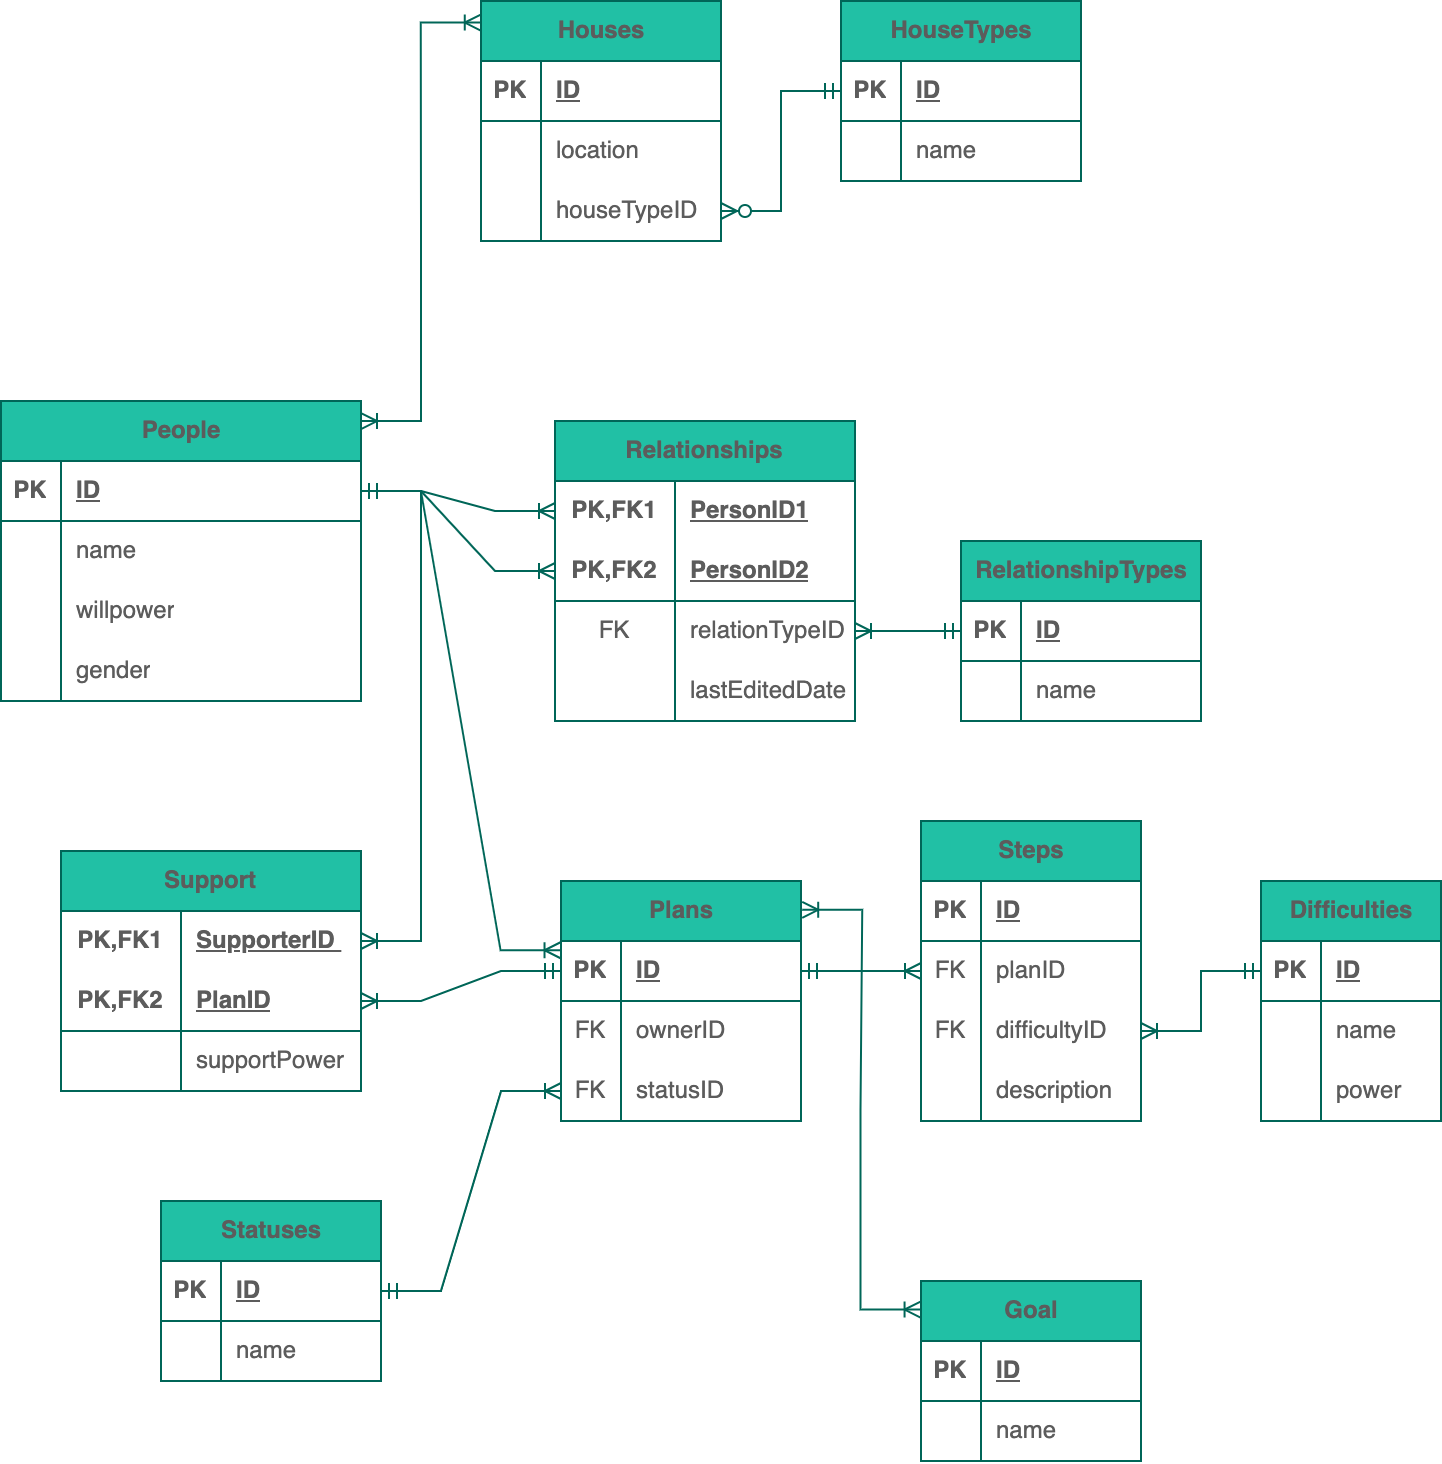
\includegraphics[width=\textwidth]{image/Infological-model.png}
\section{Даталогическая модель}
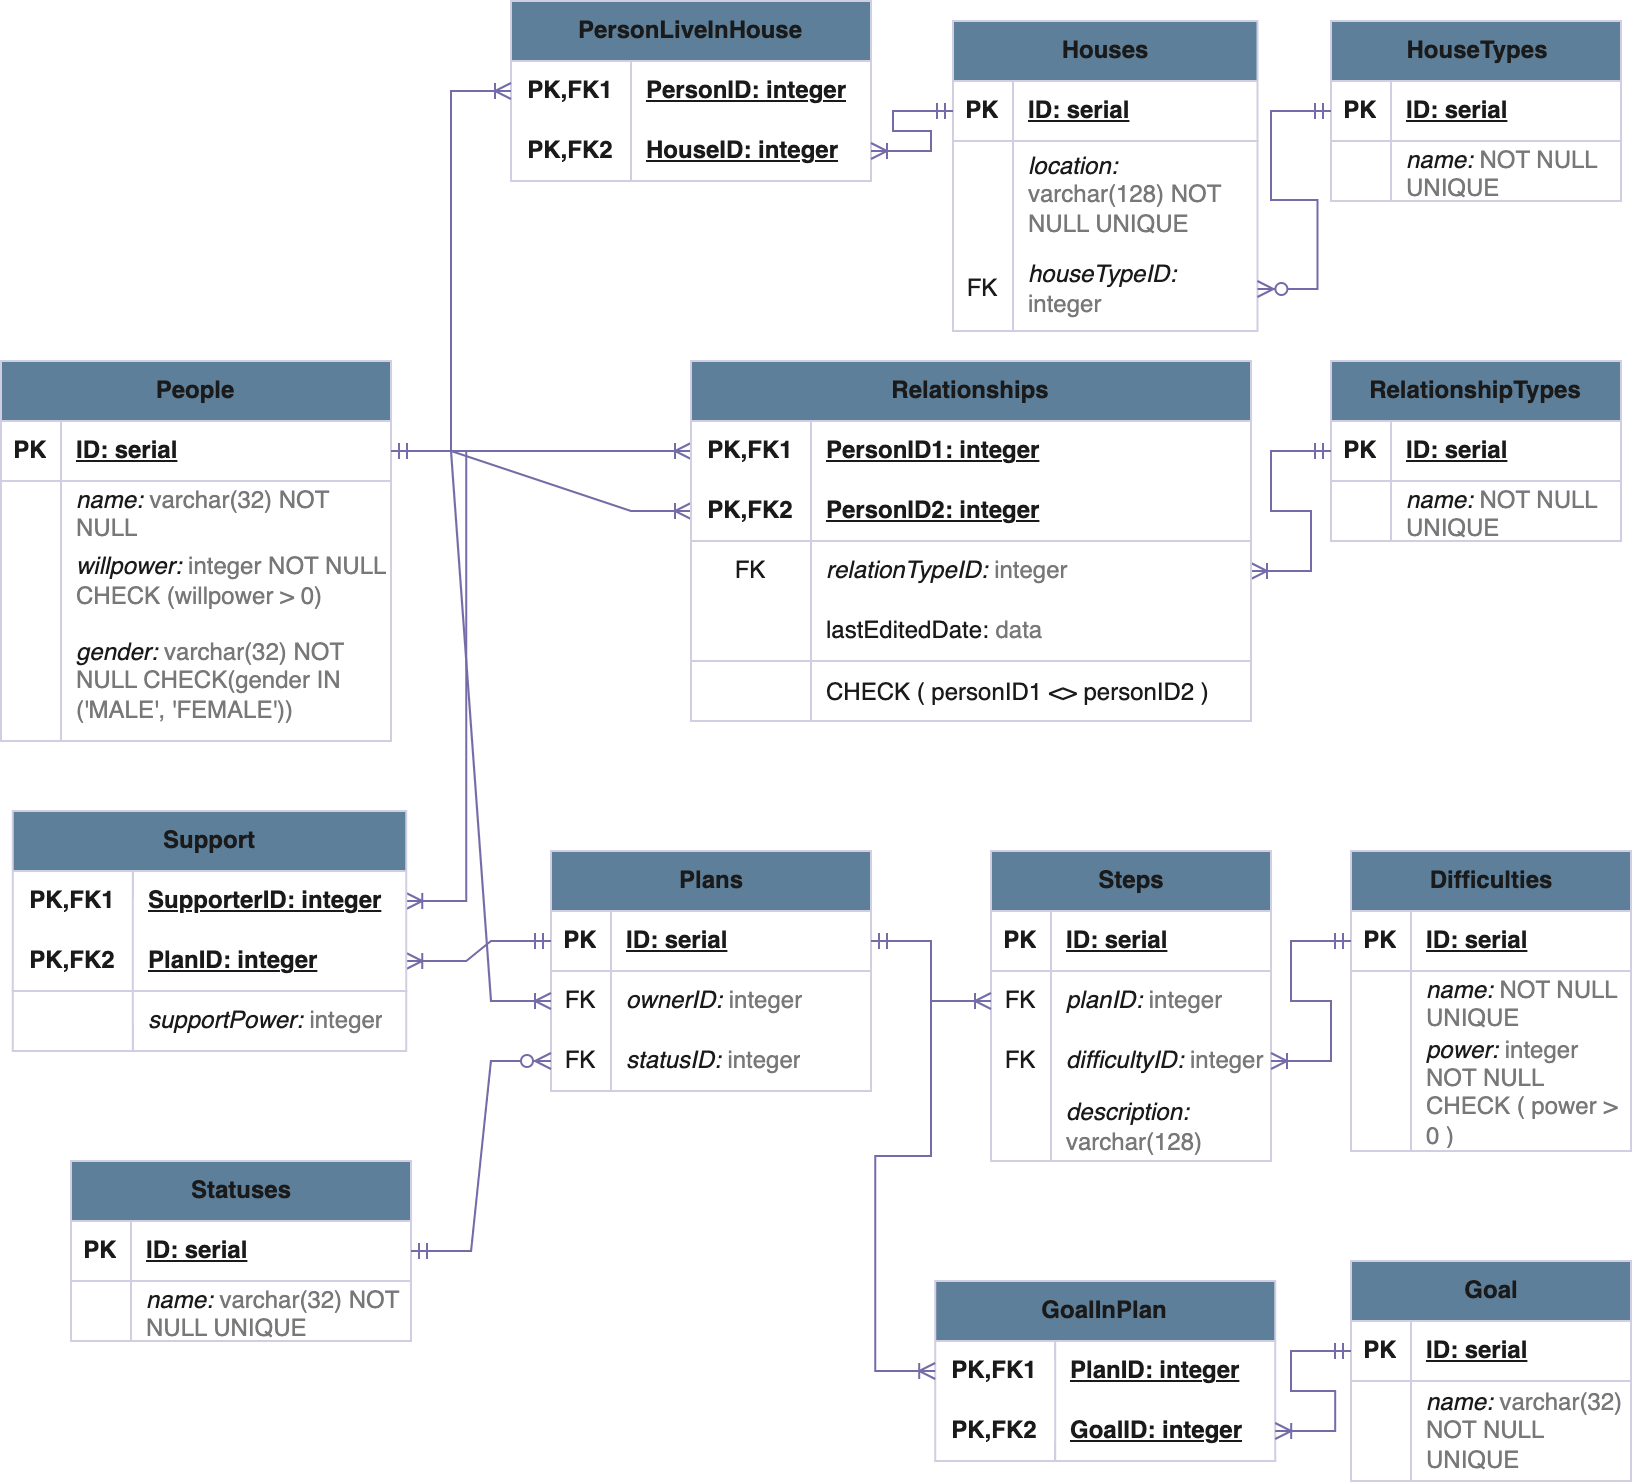
\includegraphics[width=\textwidth]{image/datalogical-model.png}
\section{Реализация даталогической модели на SQL.}
\lstdefinestyle{sql}{language=SQL, 
  basicstyle=\small\ttfamily,
  commentstyle=\color{cyan},
  stringstyle=\color{magenta}\ttfamily,
  keywordstyle=\color{blue},
  numbers=left,
  numberstyle=\scriptsize,
  numbersep=5pt,
  frame=single,
  breaklines=true,
  breakatwhitespace=true,
  showstringspaces=false,
  tabsize=4,
  inputencoding=utf8,
  extendedchars=true,
  literate={а}{{\selectfont\char224}}1
          {б}{{\selectfont\char225}}1
          {в}{{\selectfont\char226}}1
          {г}{{\selectfont\char227}}1
          {д}{{\selectfont\char228}}1
          {е}{{\selectfont\char229}}1
          {ё}{{\"e}}1
          {ж}{{\selectfont\char230}}1
          {з}{{\selectfont\char231}}1
          {и}{{\selectfont\char232}}1
          {й}{{\selectfont\char233}}1
          {к}{{\selectfont\char234}}1
          {л}{{\selectfont\char235}}1
          {м}{{\selectfont\char236}}1
          {н}{{\selectfont\char237}}1
          {о}{{\selectfont\char238}}1
          {п}{{\selectfont\char239}}1
          {р}{{\selectfont\char240}}1
          {с}{{\selectfont\char241}}1
          {т}{{\selectfont\char242}}1
          {у}{{\selectfont\char243}}1
          {ф}{{\selectfont\char244}}1
          {х}{{\selectfont\char245}}1
          {ц}{{\selectfont\char246}}1
          {ч}{{\selectfont\char247}}1
          {ш}{{\selectfont\char248}}1
          {щ}{{\selectfont\char249}}1
          {ъ}{{\selectfont\char250}}1
          {ы}{{\selectfont\char251}}1
          {ь}{{\selectfont\char252}}1
          {э}{{\selectfont\char253}}1
          {ю}{{\selectfont\char254}}1
          {я}{{\selectfont\char255}}1
          {А}{{\selectfont\char192}}1
          {Б}{{\selectfont\char193}}1
          {В}{{\selectfont\char194}}1
          {Г}{{\selectfont\char195}}1
          {Д}{{\selectfont\char196}}1
          {Е}{{\selectfont\char197}}1
          {Ё}{{\"E}}1
          {Ж}{{\selectfont\char198}}1
          {З}{{\selectfont\char199}}1
          {И}{{\selectfont\char200}}1
          {Й}{{\selectfont\char201}}1
          {К}{{\selectfont\char202}}1
          {Л}{{\selectfont\char203}}1
          {М}{{\selectfont\char204}}1
          {Н}{{\selectfont\char205}}1
          {О}{{\selectfont\char206}}1
          {П}{{\selectfont\char207}}1
          {Р}{{\selectfont\char208}}1
          {С}{{\selectfont\char209}}1
          {Т}{{\selectfont\char210}}1
          {У}{{\selectfont\char211}}1
          {Ф}{{\selectfont\char212}}1
          {Х}{{\selectfont\char213}}1
          {Ц}{{\selectfont\char214}}1
          {Ч}{{\selectfont\char215}}1
          {Ш}{{\selectfont\char216}}1
          {Щ}{{\selectfont\char217}}1
          {Ъ}{{\selectfont\char218}}1
          {Ы}{{\selectfont\char219}}1
          {Ь}{{\selectfont\char220}}1
          {Э}{{\selectfont\char221}}1
          {Ю}{{\selectfont\char222}}1
          {Я}{{\selectfont\char223}}1
}
\subsection*{Создание таблиц:}
\lstinputlisting[style=sql]{../src/tables.sql}
\subsection*{Удаление таблиц:}
\lstinputlisting[style=sql]{../src/delete.sql}
\subsection*{Заполнение тестовых значений:}
\lstinputlisting[style=sql]{../src/values.sql}
\section{Вывод}
В ходе выполнения лабораторной работы были изученны сущности и их классификация,
инфологическая модель, даталогическая модель, основы PostgreSQL.
\end{document}